% -----------------------------------------------------------------------------
\documentclass[a4paper]{artikel3}
% -----------------------------------------------------------------------------
\paperheight = 29.70 cm  \paperwidth = 21.0 cm  \hoffset        = 0.46 cm
\headheight  =  0.81 cm  \textwidth  = 15.0 cm  \evensidemargin = 0.00 cm
\headsep     =  0.81 cm	 \textheight = 9.00 in  \oddsidemargin  = 0.00 cm					
% -----------------------------------------------------------------------------
\usepackage{enumerate}
\usepackage{minted}
\usepackage{algorithm}
\usepackage{algorithmic}
\usepackage{amsfonts}
\usepackage{amsmath}
\usepackage{caption}
\usepackage{subcaption}
\usepackage{url}
\usepackage{graphicx}
\usepackage{float}
\usepackage[font=small,labelfont=bf]{caption}
\usepackage{setspace}
\usepackage{booktabs}
\usepackage[pdfpagemode=None,
		    colorlinks=true, 
		    urlcolor=blue, 
		    linkcolor=blue, 
		    citecolor=blue, 
		    pdfstartview=FitH]{hyperref}
\usepackage{pdfpages}
% -----------------------------------------------------------------------------
\newtheorem{thm}{Theorem}
\newtheorem{cor}[thm]{Corollary}
\newtheorem{lem}{Lemma}
\newtheorem{prop}{Proposition}
\newtheorem{definition}[thm]{Definition}
\newtheorem{rem}[thm]{Remark}
\newtheorem{exm}[thm]{Example}
% -----------------------------------------------------------------------------
\newcommand{\norm}[1]{\left\Vert#1\right\Vert}
\newcommand{\abs}[1]{\left\vert#1\right\vert}
\newcommand{\set}[1]{\left\{#1\right\}}
\newcommand{\Real}{\mathbb R}
\newcommand{\eps}{\varepsilon}
\newcommand{\To}{\longrightarrow}
\newcommand{\mb}[1]{\mathbf{#1}}
\newcommand{\gb}[1]{\text{\boldmath$#1$}}
\newcommand{\ov}[1]{\overline{#1}}
\newcommand{\mml}{\{}
\newcommand{\mmr}{\}}
\newcommand{\lh}[1]{\widehat{#1}}
\newcommand{\pname}[1]{\textsc{#1}}
\newcommand{\lc}[1]{\mathscr{#1}}
\newcommand{\lcs}[1]{\ov{\mathscr{#1}}}
\newcommand{\lco}[1]{\overline{\mathscr{#1}}}
\newcommand{\lch}[1]{\widehat{\mathscr{#1}}}
\newcommand{\spi}{\ell}
\newcommand{\zf}[1]{z(#1)}
\newcommand{\R}{\mathbb{R}}
% -----------------------------------------------------------------------------
\allowdisplaybreaks
\onehalfspacing
% -----------------------------------------------------------------------------

\usepackage{comment}
\begin{document}

% Title page
\begin{center}
{\Large \onehalfspacing \bf Bayesian Data Analysis course - Project work at Aalto}
\end{center}
\vspace{10pt}


\begin{center}
Thilini Panagoda, Vivian Phan, Alexandr Pimikov
\footnote{Email: pimikov@gmail.com}


\end{center}
\section{Introduction}

The assessment and control of default risk is a critical function in the ever-changing financial services industry, especially in the context of credit card lending. This study aims to identify the complex variables affecting an individual's creditworthiness within the particular setting of Taiwanese consumers' default payments. 

This report presents a comparative study of two statistical models designed to predict credit default. The first is a simple logistic regression model, and the second is a more complex hierarchical model that takes into account the educational background of credit applicants. Our goal is to determine the impact of borrowers' education on their likelihood of making timely payments. We particularly focus on the practical relevance of including educational background as a hierarchical element in the model and whether this additional complexity translates into better predictive accuracy compared to the simpler logistic regression approach.

\section{Description of the data and the analysis}

We analyze the data on default of credit card clients taken from \cite{data}. 
These data has been studied in \cite{mining,dancing}. The previous studies used machine learning methods, while we used Bayesian data analysis methods.

The data include 30000 entries on 23 explanatory variables:
\begin{itemize}
    \item Amount of the given credit (LIMIT\_BAL)
    \item Clients data (SEX, EDUCATION, MARRIAGE, AGE)
    \item History of payment (PAY\_0  PAY\_2     PAY\_3     PAY\_4     PAY\_5    PAY\_6)  
    \item Amount of bill statement (BILL\_AMT1 BILL\_AMT2 BILL\_AMT3 BILL\_AMT4 BILL\_AMT5 BILL\_AMT6 )
    \item Amount of previous payment (PAY\_AMT1  PAY\_AMT2  PAY\_AMT3  PAY\_AMT4  PAY\_AMT5  PAY\_AMT6)
    \item default payment (Yes = 1, No = 0)
\end{itemize}

\begin{comment}

\iffalse % commented
Copy past from the data cite:

Additional Variable Information

This research employed a binary variable, default payment (Yes = 1, No = 0), as the response variable. Thirds study reviewed the literature and used the following 23 variables as explanatory variables: \\
X1: Amount of the given credit (NT dollar): it includes both the individual consumer credit and his/her family (supplementary) credit. \\
X2: Gender (1 = male; 2 = female). \\
X3: Education (1 = graduate school; 2 = university; 3 = high school; 4 = others). \\
X4: Marital status (1 = married; 2 = single; 3 = others). \\
X5: Age (year). \\
X6 - X11: History of past payment. We tracked the past monthly payment records (from April to September, 2005) as follows: X6 = the repayment status in September, 2005; X7 = the repayment status in August, 2005; . . .;X11 = the repayment status in April, 2005. The measurement scale for the repayment status is: -1 = pay duly; 1 = payment delay for one month; 2 = payment delay for two months; . . .; 8 = payment delay for eight months; 9 = payment delay for nine months and above. \\
X12-X17: Amount of bill statement (NT dollar). X12 = amount of bill statement in September, 2005; X13 = amount of bill statement in August, 2005; . . .; X17 = amount of bill statement in April, 2005.  \\
X18-X23: Amount of previous payment (NT dollar). X18 = amount paid in September, 2005; X19 = amount paid in August, 2005; . . .;X23 = amount paid in April, 2005.



 X1-X5:  LIMIT\_BAL   SEX  EDUCATION MARRIAGE  AGE   
 X6-X11:: PAY\_0  PAY\_2     PAY\_3     PAY\_4     PAY\_5    PAY\_6     
 X12-X17: BILL\_AMT1 BILL\_AMT2 BILL\_AMT3 BILL\_AMT4 BILL\_AMT5 BILL\_AMT6 
 X18-X23: PAY\_AMT1  PAY\_AMT2  PAY\_AMT3  PAY\_AMT4  PAY\_AMT5  PAY\_AMT6  
 Y default  

\fi
\end{comment}

\begin{figure}
    \centering
    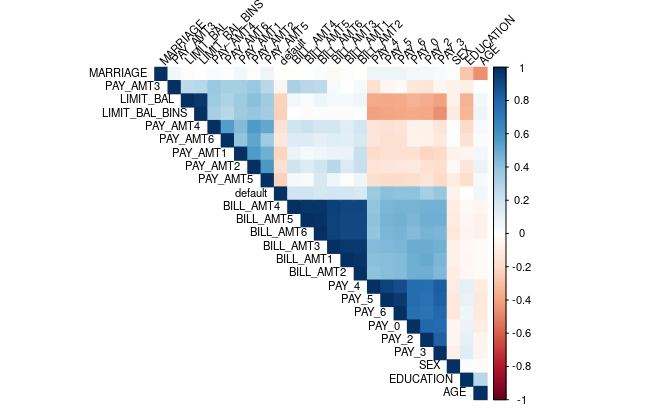
\includegraphics[width=1\linewidth]{correl_matrix.png}
    \caption{Correlation Matrix Plot}
    \label{fig:correl_matrix}
\end{figure}

The correlation matrix plot provides a visual representation of the relationships between different features in the dataset. The attribute of interest, 'default', which represents the outcome we aim to predict, shows varying degrees of correlation with different features. Notably, it exhibits a significant correlation with the 'PAY' attributes, which represent the repayment status in past periods. Among these, 'PAY\_0' and 'PAY\_2' emerge as the most strongly correlated with 'default', suggesting their higher predictive power for the outcome variable. Consequently, these two features have been selected for further analysis.

In addition to the payment history, background attributes like 'SEX', 'EDUCATION', and 'AGE' are considered. 'EDUCATION' stands out as the attribute most correlated with both 'PAY\_0' and 'PAY\_2'. This insight has guided the decision to stratify the hierarchical model by levels of education, hypothesizing that educational background may interact with repayment behavior in predicting default.

Our analysis focuses on a small sampled subset of the data, ensuring representation across different educational backgrounds (1 for graduate school, 2 for university, 3 for high school, 4 for others) and default outcomes (0 for no default, 1 for default). For each category within education and default status, we sampled 40 data points, culminating in a dataset of 240 points. This approach allows for a balanced view across the spectrum of educational attainment and repayment performance.

The models were initially fitted using this compact dataset to capture the nuances of the relationship between education level, recent payment history, and default likelihood. Post model fitting, we proceeded to validate our findings on the full dataset, comprising 30,000 entries. This step is crucial to ascertain the model's robustness and its generalizability to a broader population.

\section{Description of two models} 

We use two models: the pooled model and hierarchical  model. 
Our pooled model has the following form
\begin{align*}
    &\mu = \text{logistic}(\beta_0 + \beta_1 * \text{PAY\_0} + \beta_2 * \text{PAY\_2})\,, \\\nonumber
    &d \sim \text{Bernoulli}(\mu)
\end{align*}
where logistic function
\begin{align*}
    \text{logistic}(x) = \frac{1}{1+exp(-x)}\,,
\end{align*}
and $d$ stays for default.
Hierarchical model has one extra layer for intercept grouped by education $i = 1,2,3$:
\begin{align*}
    &d_i \sim \text{Bernoulli}(\mu_i) \\\nonumber
    &\mu_i = \text{logistic}(\beta_0 + \beta_1 * \text{PAY\_0} + \beta_2 * \text{PAY\_2} + \alpha_i)\,, \\\nonumber
    &\alpha_i  \sim  \mathcal{N}(a_i,\sigma)\,.     
\end{align*}


\section{Priors selection}
\begin{table}[h!]
  \centering
  \caption{Dataset descriptions}
  \label{tab:data_description}
  \begin{tabular}{lcccc}
    \toprule
    \textbf{Dataset} & \textbf{Nof. Entries} & \textbf{Nof. 0 entries} & \textbf{Nof. 1 entries} \\
    \midrule
    Short Data & 240 entries & 120 (50\%) & 120 (50\%) \\
    Original Data & 30000 entries & 23364 (77.88\%) & 6636 (22.12\%) \\
    \bottomrule
  \end{tabular}
\end{table}

Two distinct types of priors have been employed: a non-informative prior, $\mathcal{N}(0,100)$, and a weakly informative prior, $\mathcal{N}(\log(\frac{0.7}{0.3}), 1)$. These priors are instrumental in guiding the Bayesian inference process. Below is a detailed description of each prior, along with their justifications and mathematical formulations:

\subsection{Non-Informative Prior $\mathcal{N}(0,100)$}

This prior is a normal distribution with a mean ($\mu$) of 0 and a substantial standard deviation ($\sigma$) of 100. It represents a non-informative or weakly informative stance, implying limited prior knowledge about the parameter's value.

The mean of 0 indicates no initial preference for positive or negative values of the parameter, suggesting a neutral starting point. The large standard deviation of 100 reflects significant uncertainty regarding the parameter, essentially allowing the data to primarily influence the posterior distribution.

The probability density function (PDF) for this prior is given by:
\[ \mathcal{N}(0,100): P(\theta) = \frac{1}{\sqrt{2\pi \times 100^2}} \exp\left(-\frac{(\theta - 0)^2}{2 \times 100^2}\right) \]
where \( \theta \) represents the parameter being estimated.
\begin{align*}
    \beta_i \sim \mathcal{N}(0,100)\,.
\end{align*}
where $i= 0,1,2$.

For the hierarchical model we have additional parameters, for which following noninformative priors used to pertain to group-level effects (random effects):
\begin{align*}
    & a_i \sim \text{Exponential}(0.02) \\\nonumber
    & \sigma \sim \text{Exponential}(0.02)
\end{align*}


\subsection{Weakly Informative Prior: $\mathcal{N}(\log(\frac{0.7}{0.3}), 1)$}

Regarding the datasets distribution in Table \ref{tab:data_description}, the short dataset comprises 240 entries, evenly split between the two classes of 'default' (50\% for class 0 and 50\% for class 1), providing a balanced case scenario for model training. In contrast, the full dataset contains 30,000 entries with a class imbalance, where class 0 (non-default) constitutes the majority with 77.88\%, and class 1 (default) is the minority with 22.12\%. The choice of the prior distribution for the full dataset as $\mathcal{N}(\log(\frac{0.7}{0.3}), 1)$ is reflective of this observed class distribution. The log transformation within the normal distribution's mean parameter is an attempt to adjust for the skewness towards the majority class, potentially improving the model's ability to predict the less frequent event of 'default'.

This prior is a normal distribution centered around the natural logarithm of the odds ratio derived from a known class distribution (70\% vs. 30\%). It has a standard deviation of 1, indicating moderate confidence in this prior belief.

 
The PDF for this prior is:
\[ \mathcal{N}(log( \frac{0.7}{0.3}), 1): P(\theta) = \frac{1}{\sqrt{2\pi}} \exp\left(-\frac{(\theta - \log(\frac{0.7}{0.3}))^2}{2}\right) \]
\begin{align*}
    \beta_i \sim \mathcal{N}(\frac{0.7}{0.3},1)\,, \\
    \beta_0 \sim \mathcal{N}(0,10)\,.
\end{align*}
where $i= 1,2$.

The performance of both priors are quite similar (report further below in Sensitivity analysis). Therefore, the report will concentrate only on the prior $\mathcal{N}(0, 100)$

\section{MCMC inference}
In the pooled model, we use 4 chains in total, each with 2000 iterations  and 1000 warm-up iterations.

In the hierarchical model, in order to to reduce the value of $\hat R$ from 1.02 for case of hierarchical model we increased the number of iterations to 5000 and warmup up to 2500.  

\subsection{Rhat and ESS value for convergence diagnostic}
Convergence diagnostic is summarized in table \ref{tab:diag-pooled} for the pooled model  and table \ref{tab:diag-hier} for the hierarchical model. 
\begin{table}[ht]
\centering
\begin{tabular}{rlrrrrrrrrr}
  \hline
 & variable & mean & median & sd & mad & q5 & q95 & rhat & ess\_bulk & ess\_tail \\ 
  \hline
1 & b\_Intercept & -0.21 & -0.21 & 0.15 & 0.15 & -0.46 & 0.03 & 1.00 & 2592.41 & 2472.17 \\ 
  2 & b\_PAY\_0 & 0.52 & 0.52 & 0.15 & 0.16 & 0.28 & 0.78 & 1.00 & 2058.43 & 2543.86 \\ 
  3 & b\_PAY\_2 & 0.16 & 0.16 & 0.13 & 0.13 & -0.05 & 0.38 & 1.00 & 2074.70 & 2361.45 \\ 
  4 & lprior & -16.57 & -16.57 & 0.00 & 0.00 & -16.57 & -16.57 & 1.00 & 2417.79 &  \\ 
  5 & lp\_\_ & -158.24 & -157.93 & 1.21 & 0.98 & -160.77 & -156.90 & 1.00 & 1876.25 & 2311.99 \\ 
   \hline
\end{tabular}
\caption{Pooled model}
  \label{tab:diag-pooled}
\end{table}

%\vspace{10mm}
% latex table generated in R 4.3.1 by xtable 1.8-4 package
% Sun Dec  3 09:58:41 2023
\begin{table}[ht]
\centering
\begin{tabular}{rlrrrrrrrrr}
  \hline
 & variable & mean & median & sd & mad & q5 & q95 & rhat & ess\_bulk & ess\_tail \\ 
  \hline
1 & b\_I & -0.42 & -0.39 & 0.74 & 0.36 & -1.50 & 0.63 & 1.01 & 505.62 & 232.77 \\ 
  2 & b\_PAY\_0 & 0.22 & 0.23 & 0.17 & 0.16 & -0.05 & 0.51 & 1.00 & 1088.72 & 281.44 \\ 
  3 & b\_PAY\_2 & 0.59 & 0.59 & 0.15 & 0.15 & 0.34 & 0.84 & 1.01 & 818.61 & 305.30 \\ 
  4 & sd\_E\_\_I & 0.94 & 0.56 & 1.11 & 0.53 & 0.06 & 3.39 & 1.01 & 738.04 & 291.92 \\ 
  5 & r\_E[1,I] & 0.32 & 0.21 & 0.77 & 0.39 & -0.64 & 1.50 & 1.01 & 482.44 & 232.87 \\ 
  6 & r\_E[2,I] & -0.06 & -0.04 & 0.74 & 0.35 & -1.14 & 0.98 & 1.01 & 520.36 & 237.73 \\ 
  7 & r\_E[3,I] & -0.20 & -0.16 & 0.76 & 0.36 & -1.39 & 0.80 & 1.01 & 544.38 & 239.68 \\ 
  8 & lprior & -20.50 & -20.50 & 0.02 & 0.01 & -20.55 & -20.49 & 1.01 & 736.76 & 292.70 \\ 
  9 & lp\_\_ & -158.56 & -158.26 & 2.45 & 2.36 & -163.03 & -155.07 & 1.00 & 1481.31 & 1861.92 \\ 
   \hline
\end{tabular}
% E = EDUCATION 
% I = Intercept
  \caption{Hierarchical model.% Shortened Notation for Variable Names
  }
  \label{tab:diag-hier}
\end{table}

For the pooled model, The Rhat values for all parameters are at 1.00, which is ideal. An Rhat value of 1.00 indicates that between-chain variance is comparable to within-chain variance, suggesting that the chains have mixed well and convergence has been reached.

 The ESS values for the main parameters (b\_Intercept, b\_PAY.0, b\_PAY.2) are all above 2000, which is typically considered sufficient for reliable estimates. A higher ESS value indicates that the effective information drawn from the posterior distribution is substantial, reducing the uncertainty of the estimates.

The tail ESS values are also high, particularly for the intercept and PAY\_0, indicating that the estimation of the tail areas of the posterior distribution is reliable, which is important for accurate quantile estimation.


The hierarchical model also shows good convergence with Rhat value at 1.01 for all parameters. And the ESS values are between $\sim$500 to $\sim$1500 that leads to less precise estimates of the posterior means.

\subsection{HMC convergence diagnostics}

It can be seen from Figure \ref{fig:mcmc_models} that the pooled model converges without any issues. The off-diagonal scatter plots show no red points, indicating there were no divergent transitions during sampling, which is a positive sign for convergence. The diagonal histograms show the marginal posterior distributions for each parameter, which appear to be roughly normally distributed, suggesting no issues with skewness or multimodality.

However, the hierarchical model reveals a significant number of red points, indicating a number of divergent transitions. This is a potential sign of issues with convergence, indicating that the sampler may have struggled to explore the posterior distribution effectively.

The red points are scattered across the parameter space, which could suggest that the step size might be too large or that the model may have areas of problematic geometry that are causing the HMC sampler to diverge.

The elongation in scatter plots, especially for b\_PAY\_2, is more pronounced here, suggesting stronger correlations between some parameters. The presence of divergences in these plots indicates that these correlations may be contributing to the difficulty the sampler is experiencing.

\begin{figure}[htbp]
  \centering
  % First image (MCMC Pooled Model)
  \begin{subfigure}[b]{0.48\textwidth}
    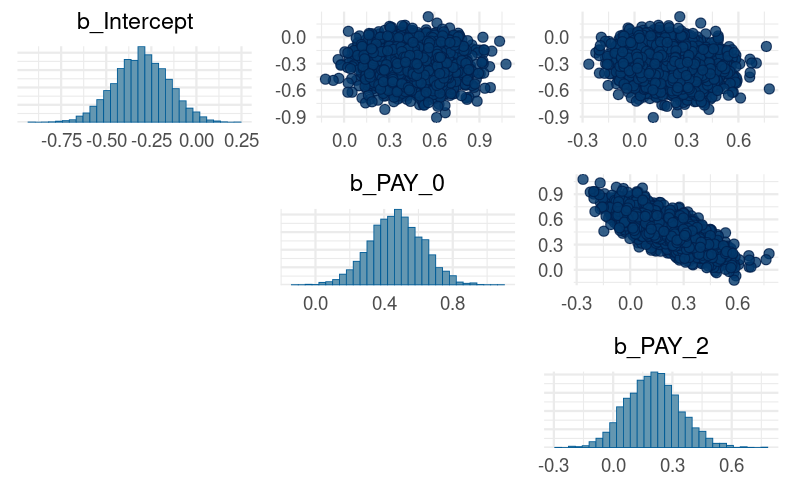
\includegraphics[width=\textwidth]{mcmc_pooled.png}
    \caption{MCMC diagnostics for the pooled model}
    \label{fig:mcmc_pooled}
  \end{subfigure}
  \hfill % This will insert a space between the two figures
  % Second image (MCMC Hierarchical Model)
  \begin{subfigure}[b]{0.48\textwidth}
    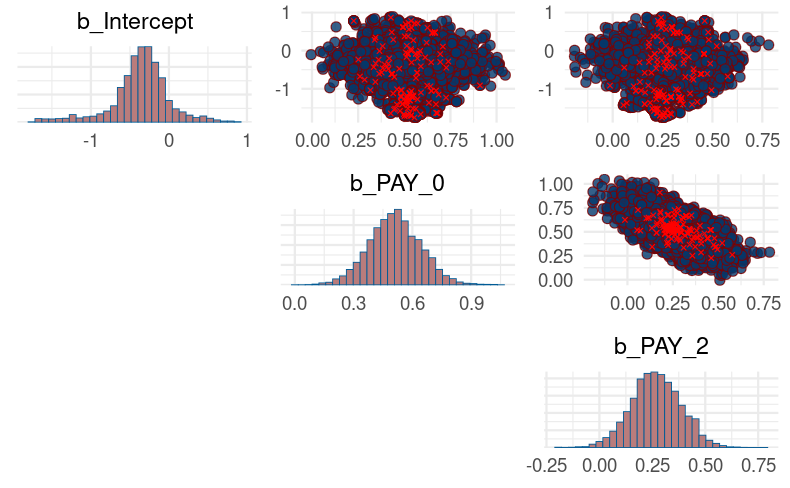
\includegraphics[width=\textwidth]{mcmc_hier.png}
    \caption{MCMC diagnostics for the hierarchical model}
    \label{fig:mcmc_hier}
  \end{subfigure}
  \caption{Comparative MCMC diagnostics for pooled and hierarchical models}
  \label{fig:mcmc_models}
\end{figure}



\section{Posterior predictive checks}
\subsection{PPC for the pooled model}
\begin{figure}[htbp]
  \centering
  \begin{subfigure}[b]{0.45\textwidth}
    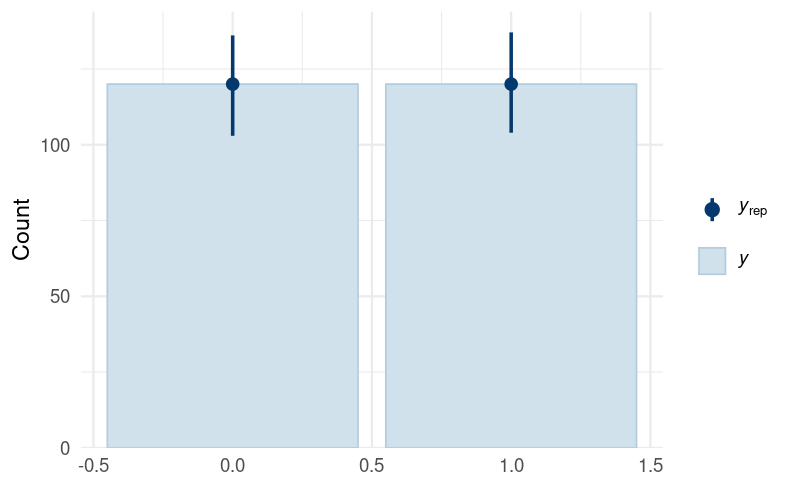
\includegraphics[width=\textwidth]{ppc_log_2.png}
    \caption{Posterior Predictive Check for Proportions}
    \label{fig:ppc_proportions}
  \end{subfigure}
  \hfill % this will insert a space between the two figures
  \begin{subfigure}[b]{0.45\textwidth}
    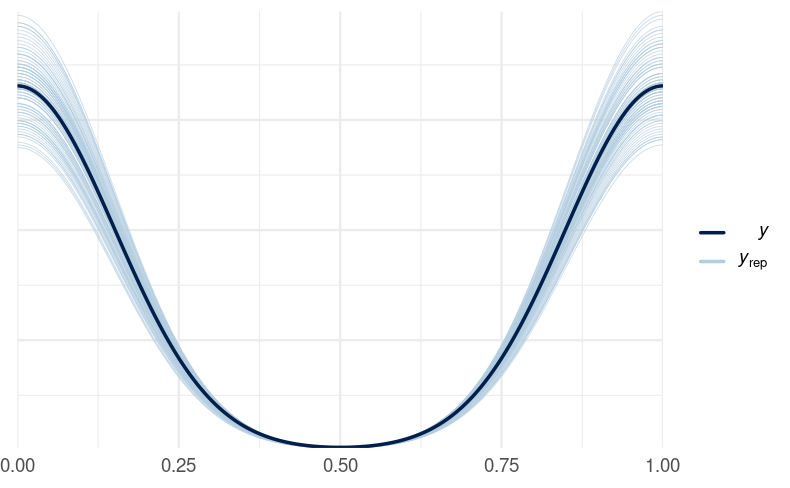
\includegraphics[width=\textwidth]{ppc_log_1.png}
    \caption{Posterior Predictive Check for Predicted Probabilities}
    \label{fig:ppc_probabilities}
  \end{subfigure}
  \caption{Posterior predictive checks using pooled model. Figure (a) presents the comparison of observed counts to the posterior predictions. Figure (b) overlays the observed proportion densities on the predicted proportion densities.}
  \label{fig:ppc_checks}
\end{figure}

The Figure \ref{fig:ppc_proportions} shows the observed counts of the binary outcomes compared to the counts from replicated datasets drawn from the posterior predictive distribution. The blue bars represent the observed data (y), and the black dots with error bars represent the median and variability (usually 50\% and 95\% intervals) of the predicted counts (y\_rep) from the posterior predictive distribution.

The fact that the observed counts fall within the range of the posterior predictive intervals for both categories suggests that the model has a reasonable fit. It does not appear to be systematically overestimating or underestimating the frequency of either outcome.

Figure \ref{fig:ppc_probabilities} overlays the density of the observed data on the densities of several replicated datasets (predictions) from the posterior predictive distribution.

The dark line represents the observed proportions (y), while the lighter lines represent the densities of predicted proportions (y\_rep) across different samples from the posterior distribution.

The close alignment of the predicted densities around the observed proportions suggests that the model is capturing the underlying distribution of the data well. 

\subsection{PPC for the hierarchical model}
\begin{figure}[htbp]
  \centering
  \begin{subfigure}[b]{0.45\textwidth}
    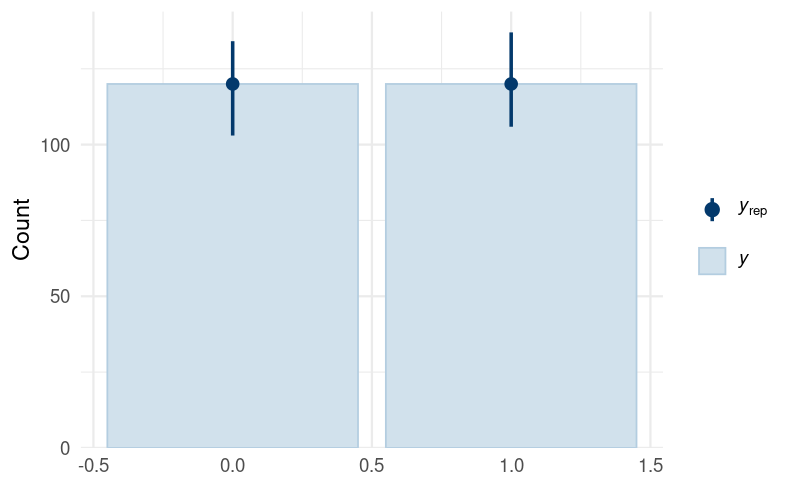
\includegraphics[width=\textwidth]{ppc_hier_1.png}
    \caption{Posterior Predictive Check for Proportions}
    \label{fig:ppc_proportions_2}
  \end{subfigure}
  \hfill % this will insert a space between the two figures
  \begin{subfigure}[b]{0.45\textwidth}
    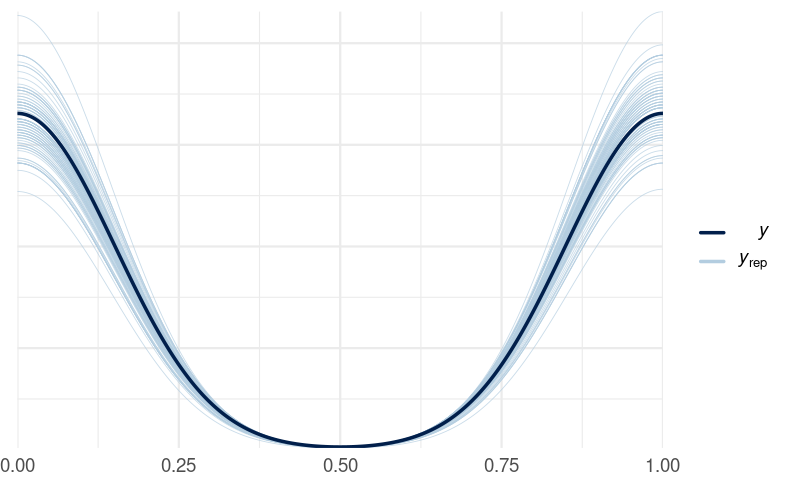
\includegraphics[width=\textwidth]{ppc_hier_2.png}
    \caption{Posterior Predictive Check for Predicted Probabilities}
    \label{fig:ppc_probabilities_2}
  \end{subfigure}
  \caption{Posterior predictive checks using hierarchical model. Figure (a) presents the comparison of observed counts to the posterior predictions. Figure (b) overlays the observed proportion densities on the predicted proportion densities.}
  \label{fig:ppc_checks_2}
\end{figure}

We can see in Figure \ref{fig:ppc_checks_2} that the hierarchical model behaves similarly as the pooled model. The predicted density follows very closely with the observed data as well as the observed counts fall within the range of the posterior predictive intervals for both categories. Therefore, we can conclude that both model behave similarly and both predict quite well the observe data.

\section{Predictive performance assessment}
\begin{comment}
Optional/Bonus: Predictive performance assessment if applicable (e.g. classification accuracy) and evaluation of practical usefulness of the accuracy. This should be reported for all models.

Pooled model for short data (240 entries) used for fitting has the  classification accuracy : 0.7542 , 95\% CI : (0.6947, 0.8073), No Information Rate : 0.5  

Pooled model for original (unclean data set , 30000 entries ) has classification accuracy: 
Accuracy : 0.81, 95\% CI : (0.8055, 0.8144),  No Information Rate : 0.7788 

Hierarchical model for short data (240 entries) used for fitting has the 
classification accuracy : 0.7458, 95\% CI : (0.6858, 0.7997), that much higher than No Information Rate : 0.5.

Hierarchical model for original (unclean data set , 30000 entries ) has classification accuracy: 0.81, 95\% CI : (0.8048, 0.8137) while no Information Rate : 0.7788.

\end{comment}
Based on the Table \ref{tab:performance}, which compares the predictive performance of pooled and hierarchical models using both short data (240 entries) and original data (30,000 entries), several points can be drawn about the practical usefulness of the accuracy reported:

\textbf{Accuracy Levels:}
Both models achieve the same accuracy with the original data set (0.80), which is quite high and indicates that either model could be practically useful for making predictions on this data. For the short data, the hierarchical model (0.75) performs slightly better than the pooled model (0.73). 

\textbf{Confidence Intervals (CI):}
The confidence intervals for the original data are narrower than those for the short data, which is expected due to the larger sample size providing more information and thus greater precision in the estimate of accuracy.
The overlap in the 95\% CIs for both models with the original data suggests no significant difference in performance between the pooled and hierarchical models at the 0.80 accuracy level.

\textbf{Practical Usefulness:}
The noninformative rate (0.7788) for the original data suggests that if a model were to predict 'no default' for all cases, it would be correct approximately 77.88\% of the time due to class imbalance. Any predictive model used in this context must significantly outperform this baseline to be considered practically useful.

The reported accuracies of 0.80 for both the pooled and hierarchical models with the original data represent only a slight improvement over the noninformative rate. This raises the question of whether the model is truly capturing the underlying risk factors for default or primarily reflecting the imbalance in the dataset.

\begin{table}[h!]
  \centering
  \caption{Predictive Performance of Models with prior $\mathcal{N}(0, 100)$. The last column is the noninformative rate, the ratio of zeros to number of data points.}
  \label{tab:performance}
  \begin{tabular}{lcccc}
    \toprule
    \textbf{Model} & \textbf{Data Type} & \textbf{Accuracy} & \textbf{95\% CI} & \textbf{Rate} \\
    \midrule
    Pooled & Short Data (240 entries) & 0.73 & (0.668, 0.784) & 0.5 \\
    Pooled & Original Data (30000 entries) & 0.80 & (0.806, 0.814) & 0.7788 \\
    \addlinespace
    Hierarchical & Short Data (240 entries) & 0.75 & (0.695, 0.807) & 0.5 \\
    Hierarchical & Original Data (30000 entries) & 0.80 & (0.795, 0.804) & 0.7788 \\
    \bottomrule
  \end{tabular}
\end{table}

\begin{figure}[htbp]
  \centering
  % PSIS plot for the pooled model
  \begin{subfigure}[b]{0.48\textwidth}
    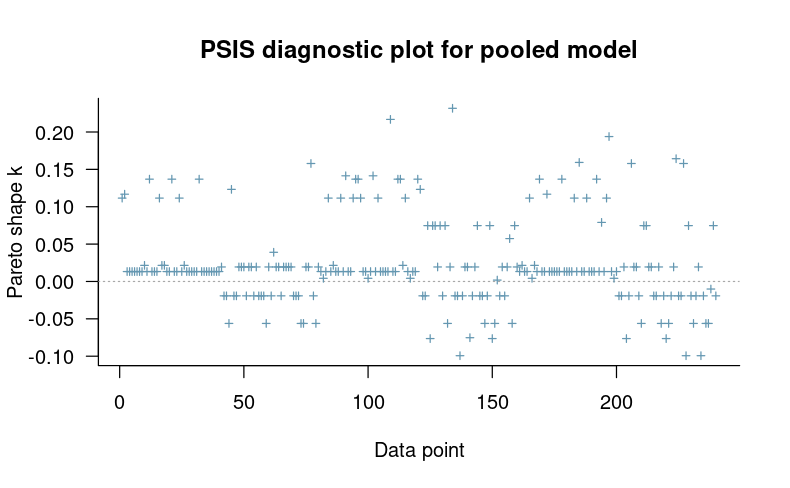
\includegraphics[width=\textwidth]{psis_pooled.png}
    \caption{PSIS diagnostic plot for the pooled model}
    \label{fig:psis_pooled}
  \end{subfigure}
  \hfill % This will insert a space between the two figures
  % PSIS plot for the hierarchical model
  \begin{subfigure}[b]{0.48\textwidth}
    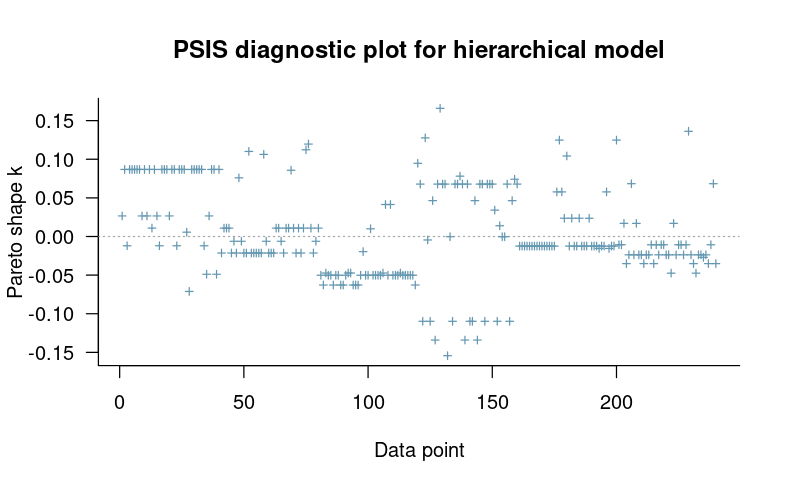
\includegraphics[width=\textwidth]{psis_hier.png}
    \caption{PSIS diagnostic plot for the hierarchical model}
    \label{fig:psis_hier}
  \end{subfigure}
  \caption{Pareto Smoothed Importance Sampling (PSIS) diagnostics for pooled and hierarchical models}
  \label{fig:both_psis}
\end{figure}

The PSIS diagnostic plots in Figure \ref{fig:both_psis} show the Pareto k-values for each observation in the model, which assess the reliability of the variational inference used in approximating the posterior distribution.

All the Pareto k-values seem to be well below 0.7, which is generally considered good. Values below 0.5 are typically seen as indicating no issues, and all the points in both the pooled model and the hierarchical plot fall under this threshold. Both models do not exhibit signs of problematic importance weights, suggesting that the variational approximations of the posterior distributions are reliable for both models.

\section{Sensitivity analysis}
\begin{table}[h!]
  \centering
  \caption{Predictive Performance of Models with prior $\mathcal{N}(\log(\frac{0.7}{0.3}), 1)$}
  \label{tab:performance_log}
  \begin{tabular}{lcccc}
    \toprule
    \textbf{Model} & \textbf{Data Type} & \textbf{Accuracy} & \textbf{95\% CI} & \textbf{Rate} \\
    \midrule
    Pooled & Short Data (240 entries) & 0.73 & (0.673, 0.788) & 0.5 \\
    Pooled & Original Data (30000 entries) & 0.81 & (0.804, 0.813) & 0.7788 \\
    \addlinespace
    Hierarchical & Short Data (240 entries) & 0.77 & (0.712, 0.822) & 0.5 \\
    Hierarchical  & Original Data (30000 entries) & 0.80 & (0.804, 0.813) & 0.7788 \\
    \bottomrule
  \end{tabular}
\end{table}

It can be observed from Table \ref{tab:performance} and Table \ref{tab:performance_log}, the model's accuracy on the short data (240 entries) and the original data (30000 entries) are reported alongside their 95\% confidence intervals (CI) and a non-informative rate. The non-informative rate is calculated as the ratio of zeros to the number of data points, providing insight into the sparsity of the dataset.

From the results, we observe only minor differences in accuracy for the short data set across the two priors, with the normal prior resulting in slightly higher accuracy. However, for the original data set, the accuracy remains the same regardless of the prior used. This might be due to the large size of the dataset, therefore, the choice of prior has a negligible effect on the model's performance. The data's strength and consistency overpower the prior's influence, indicating that the data is the main driver of the results. Moreover, the consistency in accuracy for the original data set across different priors may imply that the model is relatively insensitive to the prior specifications. 

Overall, these results indicates that for the given logistic regression models, the prior has a minor impact on the performance with a compact data set and virtually no impact with a full data set.

\section{Model comparison}

The Table \ref{tab:model_compare} shows that the hierarchical model (fit2) has an elpd\_diff of 0, which serves as the baseline, and the pooled model (fit1) has a lower elpd\_diff, indicating that it has a worse predictive performance than the hierarchical model by 7.72 points.

The se\_diff is the standard error of the difference in ELPD. The pooled model has a se\_diff of 12.17, which indicates the uncertainty associated with the elpd\_diff. 

The LOO information criterion, a measure for model comparison with a penalty for model complexity. The hierarchical model has a lower looic (272.32) compared to the pooled model (287.76), indicating better predictive performance when the complexity is accounted for.

Therefore, the hierarchical model (fit2) shows better predictive performance compared to the pooled model (fit1), as indicated by the higher elpd\_loo and the lower looic.

\begin{table}[ht]
\centering
\caption{Comparison between pooled and hierarchical model}
\begin{tabular}{rrrrrrrrr}
  \hline
 & elpd\_diff & se\_diff & elpd\_loo & se\_elpd\_loo & p\_loo & se\_p\_loo & looic & se\_looic \\ 
  \hline
fit2 & 0.00 & 0.00 & -136.16 & 7.88 & 4.92 & 0.43 & 272.32 & 15.77 \\ 
  fit1 & -7.72 & 12.17 & -143.88 & 9.39 & 4.27 & 0.98 & 287.76 & 18.77 \\ 
   \hline
\end{tabular}
\label{tab:model_compare}
\end{table}

\begin{comment}
    
\begin{table}[ht]
\centering
\caption{Comparison between pooled and hierarchical model}
\begin{tabular}{rrrrrrrrr}
  \hline
 & elpd\_diff & se\_diff & elpd\_loo & se\_elpd\_loo & p\_loo & se\_p\_loo & looic & se\_looic \\ 
  \hline
fit1 & 0.00 & 0.00 & -145.97 & 6.64 & 3.19 & 0.30 & 291.95 & 13.28 \\ 
  fit2 & -2.18 & 1.79 & -148.15 & 6.72 & 7.89 & 0.77 & 296.30 & 13.44 \\ 
   \hline
\end{tabular}
\end{table}

\end{comment}

\section{Discussion of issues and potential improvements}

\textbf{Model Accuracy vs. No Information Rate:}
Both models' accuracies do not significantly outperform the no information rate. This suggests that the models might be doing little more than predicting the most common class. For credit default prediction, this is particularly concerning because it may lead to a high rate of false negatives, where defaults are not predicted, potentially resulting in substantial financial risk.
The similar accuracy levels of both models to the no information rate could also indicate that key predictive variables or interactions are missing from the models, or that the data contains a lot of noise, which the current model structures are not capturing.

\textbf{Divergences in the Hierarchical Model:}
The presence of divergent transitions in the hierarchical model is a significant issue as it suggests problems with exploring the parameter space. This can lead to parts of the space being underexplored, potentially resulting in biased estimates or overconfidence in the model's predictions.
Divergences might also imply that the model's current parametrization is challenging for the HMC algorithm, possibly due to complex posterior geometry or highly correlated parameters.

\textbf{Comparative Performance of Models:}
Despite the hierarchical model's ability to account for group-level variability, it does not significantly outperform the pooled model in terms of accuracy. This could mean that the added complexity of the hierarchical model is not translating into better predictive performance for the data at hand, or that both models are equally limited by other factors such as data quality or feature selection.

To address divergences in the hierarchical model, consider reparameterizing the model. Non-centered parameterizations are often helpful for hierarchical models as they can reduce parameter correlations and improve sampler efficiency.

Because the dataset is imbalanced, techniques such as resampling, synthetic data generation (e.g., SMOTE) can also be used to further improve the model predictability as well.
\section{Conclusion}

In summary, our findings indicate that both models perform comparably in terms of accuracy. However, the practical utility of these models is called into question by their performance relative to the no-information rate, suggesting that the predictive power of both models is not substantially better than a naive classification by the most frequent outcome.

The hierarchical model, despite its sophisticated approach to incorporating educational background, must be approached with caution due to the presence of divergent transitions during the sampling process. These divergences highlight potential issues in the model estimation process, which could impact the reliability of its predictions.

Furthermore, the impact of priors on the model was found to be minimal. Given the large size of the dataset, the data's inherent patterns appear to overshadow the influence of the priors, rendering the choice between non-informative and weakly informative priors less consequential in the final model outcomes.

\section{Self-reflection}

During the project, the ability to perform the entire Bayesian workflow was acquired. These involve building models, selecting certain values for posterior predictive checks, and making inferences from simulations performed, in addition to utilising a variety of libraries relevant to Bayesian analysis.

Reflecting on this project, we’ve learned the importance of aligning model complexity with actual performance gains. While the hierarchical model promised a more tailored approach by considering educational background, it also introduced complexities that challenged its stability, as evidenced by the divergent transitions, underscoring the need for careful model assessment. The overwhelming influence of a large dataset on the priors highlighted the power of data in driving model results. This experience has taught us the value of rigorous model evaluation against simple benchmarks and has sharpened our approach to interpreting model diagnostics and assessing their real-world utility.


\begin{thebibliography}{9}
\bibitem{data}
https://archive.ics.uci.edu/dataset/350/default+of+credit+card+clients

\bibitem{mining}
Islam, S.R., Eberle, W.,  Ghafoor, S.K. (2018). Credit Default Mining Using Combined Machine Learning and Heuristic Approach. ArXiv, abs/1807.01176.

\bibitem{dancing}
Fung, C., Koerner, J., Grant, S., Beschastnikh, I. (2018). Dancing in the Dark: Private Multi-Party Machine Learning in an Untrusted Setting. ArXiv, abs/1811.09712.

\end{thebibliography}


\end{document} 
